% Chapter 2

%\footnote{vgl. \cite{studie}}

\renewcommand{\chaptertitle}{JavaFX - Web Application Framework}

\chapter{\chaptertitle} % Main chapter title

\label{JavaFX - Web Application Framework} % For referencing the chapter elsewhere, use \ref{Chapter1} 

\lhead{\chaptername{} \thechapter{} - \emph{\chaptertitle}} % This is for the header on each page - perhaps a shortened title

%----------------------------------------------------------------------------------------
%Review
Bevor man sich mit der eigentlichen Bewertung von JavaFX beschäftigen kann, muss zunächst erläutert werden worum es sich bei JavaFX überhaupt handelt. Dieses Kapitel dient daher als eine kurze Einführung in JavaFX, indem es zuerst der Frage nachgeht "Was ist JavaFX?". Anschließend wird der Aufbau einer typischen JavaFX-Anwendung veranschaulicht.

%----------------------------------------------------------------------------------------
%Review
\section{Was ist JavaFX?}

JavaFX wurde ursprünglich als eine neue Skripting-Plattform für Web- und Desktop-Applikationen sowie mobilen Anwendungen vorgestellt\footnote{vgl. \cite{einfuehrungInJavaFX}}, jedoch trifft diese Bezeichnung seit der Version 2.0, welche vollständig überarbeitet wurde, nicht mehr zu. Heute ist JavaFX ein auf Java-basiertes Framework zur Entwicklung von Rich Internet Applications kurz RIA und wird als eine Erweiterung von Java sowie Nachfolger von Swing angesehen\footnote{vgl. \cite{learnJavaFX8}}. JavaFX entstand als ein Lieblingsprojekt von Christopher Oliver, einem Software Engineer von Sun Microsystems, welches ursprünglich als Form Follows Function kurz F3 bekannt war. Im Jahre 2007 wurde es dann auf der JavaOne 2007 Konferenz von Sun Microsystems als JavaFX Plattform vorgestellt\footnote{vgl. \cite{beginningJavaFX}}. Diese und alle folgenden Versionen der Versionreihe 1.x basierten dabei auf der integrierten Skriptsprache JavaFX Script, daher die Bezeichnung der Skripting-Plattform (siehe Quellcode \ref{lst:JavaFXScriptExample}). Dieser Ansatz hatte jedoch nicht den gewünschten Erfolg und wurde deswegen ab JavaFX 2.0 nicht mehr zur Verfügung gestellt. Seit der Version 2.0 können JavaFX Anwendungen daher direkt in Java geschrieben werden (siehe Quellcode \ref{lst:JavaFXExample}) und bis auf den Namen hat diese Version nicht mehr viel mit der ursprünglichen gemeinsam\footnote{vgl. \cite{einfuehrungInJavaFX}}. \\

\begin{lstlisting}[language=JavaFXScript, caption=Hello World in JavaFX Script (JavaFX 1.x), frame=single, label=lst:JavaFXScriptExample]
Stage {
    title: "Hello World im alten JavaFX Script"
    width: 400
    height: 100
    scene: Scene {
        content: Text {
            font : Font { size : 32 }
            x: 0, y: 0, content: "Hello World"
        }
    } 
}
\end{lstlisting}

\begin{lstlisting}[language=Java, caption=Hello World im neuen JavaFX (ab JavaFX 2.0), frame=single, label=lst:JavaFXExample]
public void start(Stage primaryStage) throws Exception {
    primaryStage.setTitle("Hello World im aktuellen JavaFX");
    primaryStage.setWidth(400);
    primaryStage.setHeight(100);
    Label text = new Label("Hello World");
    text.setFont(new Font(32));
    Scene scene = new Scene(text);
    primaryStage.setScene(scene);
    primaryStage.show();
}
\end{lstlisting}

Seit Java SE 7 Update 6 gehört JavaFX zudem zur SE-Implementierung von Oracle sodass es nicht mehr notwendig ist zum Ausführen von JavaFX Anwendungen seperat JavaFX auf dem Gerät installiert zu haben\footnote{vgl. \cite{javafxFAQ}}. Mit Java SE 8, welches Anfang 2014 veröffentlicht wurde, wurde auch JavaFX von Version 2.x direkt auf die Version 8 erweitert um der aktuellen Java SE zu entsprechen. Des weiteren wurde dadurch JavaFX 8 zum neuen Standard für die Oberfläschen von Java Anwendungen, obwohl Swing Oberfläschen noch weiterhin unterstützt werden\footnote{vgl. \cite{javafxFAQ2}}.

Hier eine kleine Übersicht der Neuerungen in JavaFX ab der Version 2.0\footnote{vgl. \cite{javafxFAQ2}}:
\begin{itemize}
	\item Integration des aktuellen Java-Application Programming Interface (Java-API)
	\item Neue durch Hardware-beschleunigte Grafik-Pipeline Prism
	\item FXML - eine auf XML basierende Auszeichnungssprache für das Definieren von UIs
	\item Web-Komponente zum darstellen von HTML innerhalb einer Java-Anwendung
	\item Unterstützung von JavaFX in Swing und SWT, sowie von Swing in JavaFX
	\item Erstellen von eigenständigen Anwendungen mit Platform-spezifischen Installern
	\item Multi-Touch Unterstützung
	\item Neue Media-Engine mit Unterstützung von H.264 Video und AAC Audio.
	\item JavaFX Scene Builder, ein Tool zum erstellen von JavaFX UIs (wird inzwischen nicht mehr von Oracle, sondern von Gluon\footnote{\cite{gluonscenebuilder}} weiterentwickelt)
\end{itemize}


%----------------------------------------------------------------------------------------
%Review
\section{Die Architektur von JavaFX}

Im folgenden betrachten wir nun die Architektur von JavaFX, welche in Abbildung \ref{fig:jfx_architecture}\footnote{\cite{javafxarchitecture}} zu sehen ist. Diese besteht aus den JavaFX Public APIs und Scene Graph, dem Quantum Toolkit, der Grafik-Pipelines Prism und Glass Windowing Toolkit, der Media- und Web-Engine, den Grafik-Bibliotheken Java 2D, OpenGL und Direct 3D, den JDK API Libraries and Tools sowie der Java Virtual Machine. Da wir uns nur auf JavaFX konzentrieren, werden die beiden unteren Schichten wie die Java Virtual Machine und die JDK API Libraries and Tools nicht ausführlischer behandelt, da diese das Standard Java JDK darstellen.

\begin{figure}[!ht]
  \centering
    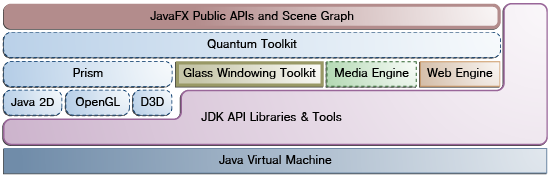
\includegraphics[width=1.0\textwidth,keepaspectratio]{images/jfx_architecture.png}\\
  \caption{JavaFX Architektur Diagramm}
  \label{fig:jfx_architecture}
\end{figure}

%----------------------------------------------------------------------------------------

\subsection{JavaFX Public APIs}

Die JavaFX Public APIs sind eine Weiterentwicklung der ursprünglichen JavaFX 1.x Produkt Linie. Der Großteil wurde dabei vollständig auf Java portiert, sodass jeder mit Java Kenntnissen diese nutzen kann um RIA Anwendungen mit JavaFX zu schreiben. Einige APIs, wie Layout und Media, wurden zusätzlich auf Basis von Feedback der Community verbessert oder simpler gestaltet. Des Weiteren nutzen die JavaFX APIs Web-Standards wie Cascading Style Sheets (CSS) und Accessible Rich Internet Applications (ARIA). Die JavaFX Public APIs stellen APIs für die RIA-Entwicklung zur Verfügung und erlauben dabei die Nutzung von Java API Features wie Generics, Annotationen und Multithreading. Weitere Features sind zudem\footnote{vgl. \cite{javafxarchitecture}}:

\begin{itemize}
	\item Erlaubt eine einfachere Nutzung von JavaFX für andere Java Virtual Machine (JVM)-basierte dynamische Sprachen wie Groovy oder JavaScript
	\item Umgekehrt erlaubt es zudem die Nutzung von Groovy oder anderen Sprachen um komplexe JavaFX Anwendungen zu schreiben
	\item Erlaubt die Nutzung von Bindings
	\item Erweitert die Java Collection Bibliothek um Observable Lists und Maps, was das Verbinden von UIs und Datenmodellen erlaubt und somit bei Änderungen im Datenmodell die UI aktualisiert.
\end{itemize}

%----------------------------------------------------------------------------------------

\subsection{Scene Graph}

Der Scene Graph ist ein hierarchischer Baum dessen Elemente Knoten (Nodes) sind. Diese stellen alle visuellen Elemente einer JavaFX Anwendung dar und ist daher der Startpunkt bei der Konstruktion einer JavaFX Anwendung. Diese Knoten können Input verarbeiten sowie gerendert werden. Die Knoten selber besitzen eine ID, eine Style class und einen Hüllkörper (Bounding volume). Des Weiteren besitzen, bis auf den Root-Knoten, alle Knoten einen Eltern-Knoten und keine oder mehrere Kind-Knoten. Dies ist in Abbildung \ref{fig:nodesfigure}\footnote{\cite{javafxscenegraph}} zu sehen, die Bezeichnung der Knoten ist dabei ein wenig geändert worden stellt aber dennoch den korrekten Scene Graph dar.

\begin{figure}[!ht]
  \centering
    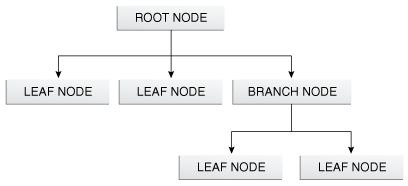
\includegraphics[width=1.0\textwidth,keepaspectratio]{images/nodesfigure.png}\\
  \caption{JavaFX Aufbau Scene Graph}
  \label{fig:nodesfigure}
\end{figure}

Zusätzlich können Knoten noch folgende Erweiterungen besitzen\footnote{vgl. \cite{javafxarchitecture}}:

\begin{itemize}
	\item Effekte, wie z.B. Schatten
	\item Deckkraft
	\item Transformationen
	\item Event handlers (für z.B. Maus-, Tasten- und Eingabe-Methoden)
	\item Einen anwendungsspezifischen Zustand (z.B. Sichtbar, Aktiviert oder Deaktiviert, usw.)
\end{itemize}

Um Inhalte zu erstellen wird die \textit{javafx.scene} API verwendet. Diese kann dabei folgende Inhalte erstellen\footnote{vgl. \cite{javafxarchitecture}}:

\begin{itemize}
	\item \textbf{Knoten (Nodes):} Formen (2D und 3D), Bilder, Medien, einen eingebetteten Web-Browser, Text, UI Controls, Diagramme, Gruppen und Container
	\item \textbf{Zustände (States):} Transformationen, visuelle Effekte und andere visuelle Zustände des Inhalts
	\item \textbf{Effekte (Effects):} Einfache Objekte, welche die Darstellung eines Scene Graph Knoten verändert, wie z.B. Schatten
\end{itemize}

%----------------------------------------------------------------------------------------

\subsection{Quantum Toolkit}

Das Quantum Toolkit dient als Bindeglied und fasst die untere Schicht mit der Grafik-Pipeline Prism, dem Glass Windowing Toolkit, sowie der Media- und Web-Engine zusammen und macht diese der JavaFX Public APIs zugänglich\footnote{vgl. \cite{einfuehrungInJavaFX}}.

%----------------------------------------------------------------------------------------

\subsection{Prism}

Prism ist eine Grafik-Pipeline zuständig für das Rendern und Berechnen von JavaFX Scenes. Es unterstützt Hardware- und Software-Rendering. Abhängig vom Betriebssystem werden dabei verschiedene Grafik-Bibliotheken verwendet\footnote{vgl. \cite{javafxarchitecture}}:

\begin{itemize}
	\item Windows XP und Windows Vista: \textbf{DirectX 9}
	\item Windows 7 und höher: \textbf{DirectX 11}
	\item Mac, Linux, Embedded: \textbf{OpenGL}
	\item Wenn Hardware-Beschleunigung nicht verfügbar ist: \textbf{Java2D Software-Rendering}
\end{itemize}

Wenn keine Hardware-Beschleunigung vorhanden ist, wird Java 2D Software-Rendering genutzt, da dieses in allen Java Runtime Environments (JRE) vorhanden ist und somit eine Anzeige gewährleistet ist. Wobei  Software-Rendering nicht die gleiche Performance erreicht wie Hardware-Rendering.

%----------------------------------------------------------------------------------------

\subsection{Glass Windowing Toolkit}

Das Glass Windowing Toolkit stellt die unterste Schicht des Grafik-Stacks von JavaFX dar. Es dient als Plattform-Abhängige Schicht und verbindet das native Betriebssystem mit JavaFX. Die Hauptfunktionalitäten sind native Betriebsservices wie das Verwalten von Fenstern, Timer und Oberfläschen. Zusätzlich verwaltet es die Event-Queues, indem es die System eigenen Event-Queue Funktionalitäten des nativen Betriebssystems nutzt. Im Gegensatz zu dem Abstract Window Toolkit (AWT) läuft es auf dem selben Thread wie die eigentliche JavaFX Anwendung\footnote{vgl. \cite{javafxarchitecture}}.

%----------------------------------------------------------------------------------------

\subsection{Media und Media Engine}

Die Media Engine stellt die Medien-Funktionalitäten für JavaFX zur Verfügung. Diese unterstützt Audio und Video mit folgenden Encoding Types, Container Types und Protokollen\footnote{\cite{javafxmedia}}:

\begin{itemize}
	\item \textbf{Encoding Types:} AAC, MP3, PCM, H.264/AVC, VP6
	\item \textbf{Container Types:} AIFF, FXM, FLV, MP3, MP4, WAV
	\item \textbf{Protokolle:} FILE, HTTP, JAR, HTTP Live Streaming (HLS)
\end{itemize}

Die Medien-Funktionalität in JavaFX wird über drei Komponenten realisiert: Einem Media-Objekt, welches die entsprechende Medien-Datei repräsentiert, einem MediaPlayer, welcher das Medium abspielt und einer MediaView, welche das Medium anzeigt. Die MediaView ist dabei jedoch nur bei Videos notwendig, da Audio direkt über den MediaPlayer läuft.

%----------------------------------------------------------------------------------------

\subsection{Web Engine}

Die Web Engine stellt die Web-Funktionalitäten für JavaFX zur Verfügung und basiert auf der Open-Source Web Browser Engine Webkit. Webkit unterstützt HTML5, CSS, JavaScript, DOM und SVG. Dadurch sind folgende Features in JavaFX Anwendungen möglich\footnote{vgl. \cite{javafxarchitecture}}:

\begin{itemize}
	\item Stellt HTML Inhalte aus lokalen oder entfernten URLs dar
	\item Unterstützt Verlauf sowie Zurück und Vorwärts Navigation
	\item Neuladen des Inhaltes
	\item Anwenden von Effekten auf die Web-Komponente
	\item Bearbeiten von HTML Inhalten
	\item Ausführen von JavaScript Befehlen
	\item Verarbeiten von Events
\end{itemize}

Die Web-Funktionalitäten werden über zwei Komponenten realisiert: der WebEngine, welche die grundlegenden Webseiten-Browsing Funktionalitäten zur Verfügung stell und der WebView, welche die Darstellung und Kontrolle der Webinhalte übernimmt.

%----------------------------------------------------------------------------------------

\subsection{Threads}

Im folgenden einen Überblick über die drei JavaFX-spezifischen Typen von Threads, welche zu jedem gegebenen Zeitpunkt einer JavaFX Anwendung laufen können\footnote{vgl. \cite{javafxarchitecture}}:

\begin{itemize}
	\item \textbf{JavaFX application thread:} Dies ist der Hauptthread einer JavaFX-Anwendung und wird für Zugriffe auf die \"{}live\"{} Scenes genutzt. \"{}Live\"{} Scenes sind Scenes, welche Teil eines Fensters sind und somit aktiv in Benutzung sind. Dadurch ist es möglich im hintergrund Scene Graphen zu erstellen ohne das die \"{}live\"{} Scenes beeinflusst werden. Erst sobald ein erstellter Scene Graph an ein \"{}live\"{} Objekt innerhalb einer \"{}live\"{} Scene angehangen wird, wird dieser selber zu einer \"{}live\"{} Scene. Der Java application thread ist jedoch eine andere Art von Thread als der typische Event Dispatch Thread (EDT) in Swing und AWT, daher muss beim einbetten von JavaFX-Code in Swing Anwendungen auf diesen Umstand geachtet werden.
	\item \textbf{Prism render thread:} Der Prism render thread verarbeitet das Rendern von Scenes unabhängig vom event dispatcher, dadurch ist es möglich einen Frame zu rendern während der nächste Frame bereits berechnet wird. Dieser Vorteil wird besondern bei Mehrkern-Prozessoren deutlich, wo zusätzlich mehrere Raster-Threads genutzt werden können um das Rendern zu beschleunigen.
	\item \textbf{Media thread:} Der Media thread läuft im Hintergrund und synchronisiert die letzten Frames durch den Scene Graph mit der Nutzung des JavaFX application threads.
\end{itemize}


%----------------------------------------------------------------------------------------
%ToDo
\section{Aufbau einer JavaFX-Anwendung}

\begin{figure}[!ht]
  \centering
    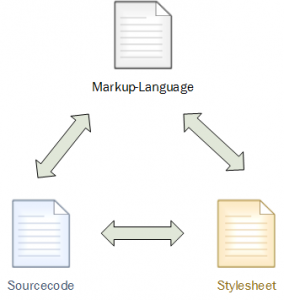
\includegraphics[width=0.5\textwidth,keepaspectratio]{images/aufbauJavaFX.png}\\
  \caption{JavaFX Aufbau einer JavaFX Anwendung}
  \label{fig:javafxaufbaufigure}
\end{figure}

%----------------------------------------------------------------------------------------

\clearpage